\documentclass[a4paper,12pt]{report}
\setcounter{secnumdepth}{5}
\setcounter{tocdepth}{3}
\input{/usr/share/LaTeX-ToolKit/template.tex}
\begin{document}
\title{Trigonometry}
\author{沈威宇}
\date{\temtoday}
\titletocdoc
\sct{Trigonometry (三角學)}
\subsection{銳角三角比(Trigonometric Ratios)的三角形定義}
\begin{itemize}
  \item 正弦(Sine,$\sin$):正弦值是對應角的對邊與斜邊之比, 即:\[\sin \theta = \frac{\text{對邊}}{\text{斜邊}}\]
  \item 餘弦(Cosine,$\cos$):餘弦值是對應角的鄰邊與斜邊之比 ,即:\[\cos \theta = \frac{\text{鄰邊}}{\text{斜邊}}\]
  \item 正切(Tangent,$\tan$):正切值是對應角的對邊與鄰邊之比,即:\[\tan \theta = \frac{\text{對邊}}{\text{鄰邊}}\]
  \item 餘切(Cotangent,$\cot$):\[\cot \theta = \frac{1}{\tan \theta}\]
  \item 正割(Secant,$\sec$):\[\sec \theta = \frac{1}{\cos \theta}\]
  \item 餘割(Cosecant,$\csc$):\[\csc \theta = \frac{1}{\sin \theta}\]
\end{itemize}
\subsection{廣義角三角比或三角函數(Trigonometric functions)的單位圓定義}
任意廣義角的三角函數值可以表示為:
\begin{itemize}
  \item 正弦(Sine,$\sin$):角 \(\theta\) 的正弦值是單位圓上 對應點的 \(y\) 坐標,即:\[\sin \theta = y\]。為奇函數,定義域$\mathbb{R}$,值域$[-1,1]$,週期$2\pi$,振幅1,線對稱於$x=\qty(n+\frac{1}{2})\pi,n\in\mathbb{Z}$,點對稱於$\qty(\qty(n\pi,n\in\mathbb{Z}),0)$。
  \item 餘弦(Cosine,$\cos$):角 \(\theta\) 的餘弦值是單位圓 上對應點的 \(x\) 坐標,即:\[\cos \theta = x\]。為偶函數,定義 域$\mathbb{R}$,值域$[-1,1]$,週期$2\pi$,振幅1,線對稱於$x=n\pi,n\in\mathbb{Z}$,點對稱於$\qty(\qty(\qty(n+\frac{1}{2})\pi,n\in\mathbb{Z}),0)$,$\cos(x)=\sin\qty(x+\frac{\pi}{2})$ 。
  \item 正切(Tangent,$\tan$):角 \(\theta\) 的正切值是正弦值與餘弦值的比,即:\[\tan \theta = \frac{\sin \theta}{\cos \theta} = \frac{y}{x}\]。為奇函數,定義域$\left\{x\in\mathbb{R}\left |\pi\nmid\qty(x-\frac{\pi}{2})\right.\right\}$,值域$\mathbb{R}$,週期$\pi$,點對稱於$\qty(\qty(\frac{n}{2}\pi,n\in\mathbb{Z}),0)$。
  \item 餘切(Cotangent,$\cot$):\[\cot \theta = \frac{1}{\tan \theta}\]。為奇函數,定義域$\left\{x\in\mathbb{R}\left |\pi\nmid x\right.\right\}$,值域$\mathbb{R}$,週期$\pi$,點對稱於$\qty(\qty(\frac{n}{2}\pi,n\in\mathbb{Z}),0)$,$\cot(x)=-\tan\qty(x+\frac{\pi}{2})$。
  \item 正割(Secant,$\sec$):\[\sec \theta = \frac{1}{\cos \theta}\]。為偶函數,定義域$\left\{x\in\mathbb{R}\left |\pi\nmid\qty(x-\frac{\pi}{2})\right.\right\}$,值域$\left\{y\in\mathbb{R}\left |-1\leq y \lor y\leq 1\right.\right\}$,週期$\pi$,線對稱於$\qty(\qty(n\pi,n\in\mathbb{Z}),0)$,點對稱於$x=\qty(n+\frac{1}{2})\pi,n\in\mathbb{Z}$。
  \item 餘割(Cosecant,$\csc$):\[\csc \theta = \frac{1}{\sin \theta}\]。為奇函數,定義域$\left\{x\in\mathbb{R}\left |\pi\nmid x\right.\right\}$,值域$\left\{y\in\mathbb{R}\left |-1\leq y \lor y\leq 1\right.\right\}$,週期$\pi$,線對稱於$x=\qty(n+\frac{1}{2})\pi,n\in\mathbb{Z}$,點對稱於$\qty(\qty(n\pi,n\in\mathbb{Z}),0)$,$\csc(x)=\sec\qty(x-\frac{\pi}{2})$。
\end{itemize}
\subsection{特殊角三角函數值}
\renewcommand{\arraystretch}{1.5}
\begin{longtable}[c]{|p{0.1\textwidth}|p{0.1\textwidth}|p{0.2\textwidth}|p{0.2\textwidth}|p{0.2\textwidth}|}
\hline
Radian & Angle & $\sin$ & $\cos$ & $\tan$ \\\hline\endhead
0 & 0° & 0 & 1 & 0 \\\hline
$\frac{\pi}{2}$ & 90° & 1 & 0 & \\\hline
$\pi$ & 180° & 0 & -1 & 0 \\\hline
$\frac{3\pi}{2}$ & 270° & -1 & 0 & \\\hline
$\frac{\pi}{4}$ & 45° & $\frac{\sqrt{2}}{2}$ & $\frac{\sqrt{2}}{2}$ & $1$ \\\hline
$\frac{3\pi}{4}$ & 135° & $\frac{\sqrt{2}}{2}$ & $-\frac{\sqrt{2}}{2}$ & -1 \\\hline
$\frac{\pi}{6}$ & 30° & $\frac{1}{2}$ & $\frac{\sqrt{3}}{2}$ & $\frac{\sqrt{3}}{3}$ \\\hline
$\frac{\pi}{3}$ & 60 ° & $\frac{\sqrt{3}}{2}$ & $\frac{1}{2}$ & $\sqrt{3}$ \\\hline
$\frac{2\pi}{3}$ & 120° & $\frac{\sqrt{3}}{2}$ & $-\frac{1}{2}$ & $-\sqrt{3}$ \\\hline
$\frac{5\pi}{6}$ & 150° & $\frac{1}{2}$ & $-\frac{\sqrt{3}}{2}$ & $-\frac{\sqrt{3}}{3}$ \\\hline
$\frac{\pi}{12}$ & 15° & $\frac{\sqrt{6}-\sqrt{2}}{4}$ & $\frac{\sqrt{6}+\sqrt{2}}{4}$ & $2-\sqrt{3}$ \\\hline
$\frac{5\pi}{12}$ & 75° & $\frac{\sqrt{6}+\sqrt{2}}{4}$ & $\frac{\sqrt{6}-\sqrt{2}}{4}$ & $2+\sqrt{3}$ \\\hline
$\frac{\pi}{10}$ & 18° & $\frac{\sqrt{5}-1}{4}$ & $\frac{\sqrt{10+2\sqrt{5}}}{4}$ & $\frac{\sqrt{5}-1}{\sqrt{10+2\sqrt{5}}}$ \\\hline
$\frac{2\pi}{10}$ & 36° & $\frac{\sqrt{10-2\sqrt{5}}}{4}$ & $\frac{\sqrt{5}+1}{4}$ & $\frac{\sqrt{10-2\sqrt{5}}}{\sqrt{5}+1}$ \\\hline
$\frac{3\pi}{10}$ & 54° & $\frac{\sqrt{5}+1}{4}$ & $\frac{\sqrt{10-2\sqrt{5}}}{4}$ & $\frac{\sqrt{5}+1}{\sqrt{10-2\sqrt{5}}}$ \\\hline
$\frac{4\pi}{10}$ & 72° & $\frac{\sqrt{10+2\sqrt{5}}}{4}$ & $\frac{\sqrt{5}-1}{4}$ & $\frac{\sqrt{10+2\sqrt{5}}}{\sqrt{5}-1}$ \\\hline
& 37° & $\approx 0.6018$ & $\approx 0.7986$ & $\approx 0.7536$ \\\hline
& 53° & $\approx 0.7986$ & $\approx 0.6018$ & $\approx 1.3270$ \\\hline
\end{longtable}
\FB
\ssc{三角函數基本關係}
\begin{center}
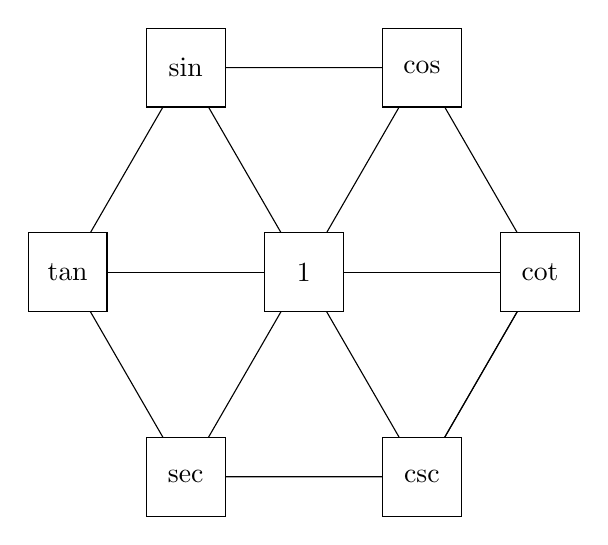
\begin{tikzpicture}
  \foreach \a in {0,60,...,300}
    \node (P\a) at (\a:3) {};
  \draw (P0) -- (P60) -- (P120) -- (P180) -- (P240) -- (P300) -- (P0) -- cycle;
  \draw (P0) -- (P180);
  \draw (P60) -- (P240);
  \draw (P120) -- (P300);
  \draw (P0) -- (P300);
  \node[draw, fill=white, minimum size=1cm, anchor=center] at (P0) {$\cot$};
  \node[draw, fill=white, minimum size=1cm, anchor=center] at (P60) {$\cos$};
  \node[draw, fill=white, minimum size=1cm, anchor=center] at (P120) {$\sin$};
  \node[draw, fill=white, minimum size=1cm, anchor=center] at (P180) {$\tan$};
  \node[draw, fill=white, minimum size=1cm, anchor=center] at (P240) {$\sec$};
  \node[draw, fill=white, minimum size=1cm, anchor=center] at (P300) {$\csc$};
  \node[draw, fill=white, minimum size=1cm, anchor=center] at (0,0) {$1$};
\end{tikzpicture}
\end{center}
\bit
\item 名稱:左側三者為正;右側三者為餘;上面二者為弦;中間二者為切;下面二者為割。
\item 餘角關係:以鉛直軸為對稱軸,位於線對稱位置者為餘角關系,即對於銳角$\theta$,左$(\theta)=$右$\qty(\frac{\pi}{2}-\theta)$。
\item 倒數關係:三條通過中心點的連線為倒數關係,其兩端者互為倒數,相乘為1。
\item 商數關係:六邊形周上,連續三個頂點形成的連線,其兩端者相乘等於中間者。
\item 平方關係:圖中有三個倒正三角形,其在上方兩頂點之二者之平方和等於在下方頂點者。
\eit
\ssc{奇變偶不變,正負看象限}
今有函數$f$,已知其為$\sin$、$\cos$、$\tan$、$\sec$、$\csc$、$\cot$之一,且已知$f(\theta)$。欲求$f(\phi)$,其中$\phi=\pm\theta\pm n\frac{\pi}{2}$,其中$n\in\mathbb{Z}$。
\bit
\item 判斷方法:奇變偶不變,正負看象限。
\item 上句:奇偶指$n$之奇偶,變指倒數,即:若$n$為奇數則令$g(\theta)=\frac{1}{f\qty(\theta)}$,否則令$g(\theta)=f(\theta)$,則$|f(\phi)|=|g(\theta)|$。
\item 下句:象限指假設$[r,\theta]$在第一象限時,$[r,\phi]$之象限。令該象限中任意角度為$\omega$。令$k=\frac{f\qty(\phi)}{g\qty(\theta)}$。則$k=\frac{f\qty(\omega)}{\qty|f(\qty(\omega)|}$,即:
\begin{center}
\begin{figure}[H]
\centering
\begin{tabular}{|p{0.16\textwidth}|p{0.16\textwidth}|p{0.16\textwidth}|p{0.16\textwidth}|p{0.16\textwidth}|}
\hline
\diagbox{$f$}{象限} & 一 & 二 & 三 & 四 \\\hline
$\sin$ & + & + & - & - \\\hline
$\cos$ & + & - & - & + \\\hline
$\tan$ & + & - & + & - \\\hline
$\csc$ & + & + & - & - \\\hline
$\sec$ & + & - & - & + \\\hline
$\cot$ & + & - & + & - \\\hline
\end{tabular}
\end{figure}\FB
\end{center}
\eit
\subsection{三角函數指數形式}
根據歐拉/尤拉公式:
\[e^{i\theta}=\cos\theta+i\sin\theta\]
三角函數可寫為:
\bma
\sin x &= \frac{e^{ix}-e^{-ix}}{2i}\\
\cos x &= \frac{e^{ix}+e^{-ix}}{2}\\
\tan x &= -i\frac{e^{2ix}-1}{e^{2ix}+1},\quad x\neq\frac{\pi}{2}+k\pi,k\in\mathbb{Z}\\
\cot x &= i\frac{e^{2ix}+1}{e^{2ix}-1},\quad x\neq k\pi,k\in\mathbb{Z}\\
\sec x &= \frac{2e^{ix}}{e^{2ix}+1},\quad x\neq\pi+2k\pi,k\in\mathbb{Z}\\
\csc x &= i\frac{2e^{ix}}{e^{2ix}-1},\quad x\neq 2k\pi,k\in\mathbb{Z}
\eam
\sct{反三角函數(Inverse trigonometric functions}
\subsection{反三角函數}
\begin{longtable}[c]{|p{0.09\textwidth}|p{0.17\textwidth}|p{0.12\textwidth}|p{0.23\textwidth}|p{0.23\textwidth}|}
\hline
名稱 & 常用符號 & 定義 & 定義域 & 值域 \\ 
\hline\endhead
反正弦 & \(y=\arcsin x\) & \(x=\sin y\) & \([-1,1]\) & \([-\frac{\pi}{2},\frac{\pi}{2}]\) \\ 
\hline
反餘弦 & \(y=\arccos x\) & \(x=\cos y\) & \([-1,1]\) & \([0,\pi]\) \\ 
\hline
反正切 & \(y=\arctan x\) & \(x=\tan y\) & \(\mathbb{R}\) & \((-\frac{\pi}{2},\frac{\pi}{2})\) \\ 
\hline
反餘切 & \(y=\arccot x\) & \(x=\cot y\) & \(\mathbb{R}\) & \((0,\pi)\) \\ 
\hline
反正割 & \(y=\arcsec x\) & \(x=\sec y\) & \((-\infty,-1]\cup[1,+\infty)\) & \([0,\frac{\pi}{2})\cup(\frac{\pi}{2},\pi]\) \\ 
\hline
反餘割 & \(y=\arccsc x\) & \(x=\csc y\) & \((-\infty,-1]\cup[1,+\infty)\) & \([-\frac{\pi}{2},0)\cup(0,\frac{\pi}{2}]\) \\ 
\hline
\end{longtable}
\FB
\subsection{atan2 函數}
$\operatorname{atan2}(y,x)$在$x>0$時返還$\tan(\theta)=\frac{y}{x}$在$(-\frac{\pi}{2},\frac{\pi}{2})$中的解,在$x<0$、$y\geq 0$時返還$\tan(\theta)=\frac{y}{x}$在$(\frac{\pi}{2},\pi)$中的解,在$x<0$、$y<0$時返還$\tan(\theta)=\frac{y}{x}$在$(-\pi,-\frac{\pi}{2})$中的解,在$x=0$、$y\neq 0$時返還$\frac{y}{\abs{y}}\frac{\pi}{2}$,在$x=y=0$時返還值未定義。
\sct{雙曲函數(Hyperbolic functions)}
\ssc{雙曲函數}
各雙曲函數之名稱均以對應之三角函數之名稱前加雙曲(hyperbolic) ,代號則為對應之三角函數代號後加 h。
\bma
\sinh x &= \frac{e^{x}-e^{-x}}{2}\\
\cosh x &= \frac{e^{x}+e^{-x}}{2}\\
\tanh x &= \frac{e^{2x}-1}{e^{2x}+1}\\
\coth x &= \frac{e^{2x}+1}{e^{2x}-1},\quad x\neq 0\\
\operatorname{sech} x &= \frac{2e^{x}}{e^{2x}+1}\\
\operatorname{csch} x &= \frac{2e^{x}}{e^{2x}-1},\quad x\neq 0
\eam
\subsection{反雙曲函數對數形式}
\bma
\operatorname{arcsinh} &= \ln\left(x+{\sqrt {x^{2}+1}}\right)\\
\operatorname{arccosh} &= \ln \left(x+{\sqrt {x^{2}-1}}\right),\quad x\geq 1\\
\operatorname{arctanh} &= \frac {1}{2}\ln \left({\frac {1+x}{1-x}}\right),\quad\abs{x}<1\\
\operatorname{arccoth} &= {\frac {1}{2}}\ln \left({\frac {x+1}{x-1}}\right),\quad\abs{x}>1\\
\operatorname{arcsech} &= \ln \left({\frac {1}{x}}+{\frac {\sqrt {1-x^{2}}}{x}}\right),\quad 0<x\leq 1\\
\operatorname{arccsch} &= \ln \left({\frac {1}{x}}+{\frac {\sqrt {1+x^{2}}}{\abs{x}}}\right),\quad x\neq 0
\eam
\sct{公式定理}
\ssc{三角函數公式}
\sssc{正切萬能公式}
\[\sin\theta=\frac{2\tan\frac{\theta}{2}}{1+\tan^2\frac{\theta}{2}}\]
\[\cos\theta = \frac{1-\tan^2\frac{\theta}{2}}{1+\tan^2\frac{\theta}{2}}\]
\[\tan\theta = \frac{2\tan\frac{\theta}{2}}{1-\tan^2\frac{\theta}{2}}\]
\sssc{二倍角公式}
\[\sin 2\theta=2\sin\theta\cos\theta\]
\bma
\cos 2\theta &=1-2\sin^2\theta\\
&=2\cos^2\theta-1\\
&=\cos^2\theta-\sin^2\theta
\eam
\sssc{半角公式與平方化倍角公式}
\bma
\sin^2\frac{\theta}{2}  &=\frac{1-\cos \theta}{2}\\
\cos^2\frac{\theta}{2}  &=\frac{1+\cos \theta}{2}\\
\tan^2\frac{\theta}{2}  &=\frac{1-\cos \theta}{1+\cos \theta}\\
\tan\frac{\theta}{2} &=\frac{\sin\theta}{1+\cos\theta}\\
&=\frac{1-\cos\theta}{\sin\theta}\\
&=\frac{1+\sin\theta-\cos\theta}{1+\sin\theta+\cos\theta}\\
&=\csc\theta-\cot\theta
\eam
\sssc{三倍角公式}
\[\sin 3\theta=3\sin\theta-4\sin^3\theta\]
\[\cos 3\theta=4\cos^3\theta-3\cos\theta\]
\[\tan 3\theta=\frac{3\tan\theta-\tan^3\theta}{1-3\tan^2\theta}\]
\sssc{和差角公式}
\[\sin\qty(\alpha +\beta)=\sin\alpha\cos\beta +\cos\alpha\sin\beta\]
\[\sin\qty(\alpha -\beta)=\sin\alpha\cos\beta -\cos\alpha\sin\beta\]
\[\cos\qty(\alpha +\beta)=\cos\alpha\cos\beta -\sin\alpha\sin\beta\]
\[\cos\qty(\alpha -\beta)=\cos\alpha\cos\beta +\sin\alpha\sin\beta\]
\[\tan\qty(\alpha +\beta)=\frac{\tan\alpha+\tan\beta}{1-\tan\alpha\tan\beta}\]
\[\tan\qty(\alpha -\beta)=\frac{\tan\alpha-\tan\beta}{1+\tan\alpha\tan\beta}\]
\[\cot\qty(\alpha +\beta)=\frac{\cot\alpha\cot\beta -1}{\cot\alpha +\cot\beta}\]
\[\cot\qty(\alpha -\beta)=\frac{\cot\alpha\cot\beta +1}{-\cot\alpha +\cot\beta}\]
\[\sec\qty(\alpha +\beta)=\frac{\sec\alpha\sec\beta \csc\alpha\csc\beta}{-\sec\alpha\sec\beta +\csc\alpha\csc\beta}\]
\[\sec\qty(\alpha -\beta)=\frac{\sec\alpha\sec\beta \csc\alpha\csc\beta}{\sec\alpha\sec\beta +\csc\alpha\csc\beta}\]
\[\csc\qty(\alpha +\beta)=\frac{\sec\alpha\sec\beta \csc\alpha\csc\beta}{\sec\alpha\sec\beta +\csc\alpha\csc\beta}\]
\[\csc\qty(\alpha -\beta)=\frac{\sec\alpha\sec\beta \csc\alpha\csc\beta}{\sec\alpha\sec\beta -\csc\alpha\csc\beta}\]
\sssc{平方關係}
\[\sin^2\theta=\frac{\tan^2\theta}{1+\tan^2\theta}=1-\cos^2\theta\]
\[\cos^2\theta=\frac{1}{1+\tan^2\theta}=1-\sin^2\theta\]
\[\tan^2\theta=\frac{1-\cos^2\theta}{\cos^2\theta}=\frac{\sin^2\theta}{1-\sin^2\theta}\]
\sssc{三角形內角正切公式}
\[\qty(\alpha+\beta+\gamma=\pi+2k\pi,\quad k\in\mathbb{Z})\iff\qty(\tan\alpha+\tan\beta+\tan\gamma=\tan\alpha\cdot\tan\beta\cdot\tan\gamma)\]
\sssc{正餘弦函數疊合}
\[\qty(a\sin\theta +b\cos\theta)^2\leq a^2+b^2,\quad a,b\in\mathbb{R}\]
\bma
a\sin x+b\cos x
&= \sqrt{a^2+b^2}\sin\qty(x+\tan^{-1}\left(\frac{b}{a}\right))\\
&= \sqrt{a^2+b^2}\cos\qty(x-\tan^{-1}\left(\frac{a}{b}\right))
\eam
\sssc{和差化積公式}
\bma
\sin\alpha +\sin\beta &= 2\sin\frac{\alpha +\beta}{2}\cos\frac{\alpha -\beta}{2}\\
\sin\alpha -\sin\beta &= 2\cos\frac{\alpha +\beta}{2}\sin\frac{\alpha -\beta}{2}\\
\cos\alpha +\cos\beta &= 2\cos\frac{\alpha +\beta}{2}\cos\frac{\alpha -\beta}{2}\\
\cos\alpha -\cos\beta &= -2\sin\frac{\alpha +\beta}{2}\sin\frac{\alpha -\beta}{2}
\eam
\sssc{積化和差公式}
\bma
2\sin\alpha\cos\beta &= \sin (\alpha +\beta)+\sin (\alpha -\beta)\\
2\cos\alpha\sin\beta &= \sin (\alpha +\beta)-\sin (\alpha -\beta)\\
2\cos\alpha\cos\beta &= \cos (\alpha +\beta)+\cos (\alpha -\beta)\\
2\sin\alpha\sin\beta &= -\cos (\alpha +\beta)+\cos (\alpha -\beta)
\eam
\sssc{連加公式}
\[\begin{aligned}
& \sum_{k=1}^{n} \sin(k\theta) = \frac{\sin\left(\frac{n\theta}{2}\right) \sin\left(\frac{(n+1)\theta}{2}\right)}{\sin\left(\frac{\theta}{2}\right)}.\\
& \sum_{k=1}^{n} \cos(k\theta) = \frac{\sin\left(\frac{n\theta}{2}\right) \cdot \cos\left(\frac{(n+1)\theta}{2}\right)}{\sin\left(\frac{\theta}{2}\right)}.
\end{aligned}\]
\sssc{正餘切和等於正餘割積公式}
\[\tan\theta+\cot\theta=\sec\theta\csc\theta\]
\sssc{正餘弦四次方和公式}
\[\sin^4\theta +\cos^4\theta = 1-2\sin^2\cos^2\theta=1-\frac{1}{2}\sin^2(2\theta)\]
\sssc{正餘弦四次方差公式}
\[\sin^4\theta -\cos^4\theta = \sin^2\theta -\cos^2\theta=-\cos(2\theta)\]
\sssc{正餘弦六次方和公式}
\[\sin^6\theta +\cos^6\theta = 1-3\sin^2\cos^2\theta=1-\frac{3}{4}\sin^2(2\theta)\]
\ssc{正弦連乘、餘切連加、餘割平方級數與餘切平方級數公式}
\[\prod_{k=0}^{n-1}\sin\qty(x+\frac{\pi k}{n})=2^{1-n}\sin\qty(nx)\]
\[\sum_{k=0}^{n-1}\cot\qty(x+\frac{\pi k}{n})=n\cot\qty(nx)\]
\[\sum_{k=0}^{n-1}\csc^2\qty(x+\frac{\pi k}{n})=n^2\csc^2\qty(nx)\]
\[\sum_{k=1}^{n-1}\csc^2\frac{\pi k}{n}=\frac{(n-1)(n+1)}{3}\]
\[\sum_{k=1}^{n-1}\cot^2\frac{\pi k}{n}=\frac{(n-1)(n-2)}{3}\]
\begin{proof}
\[\begin{aligned}
\prod_{k=0}^{n-1}\sin\qty(x+\frac{\pi k}{n})\\
&=\prod_{k=0}^{n-1}\frac{i}{2}\qty(e^{-i\qty(x+\frac{\pi k}{n})}-e^{i\qty(x+\frac{\pi k}{n})})\\
&=i^n2^{-n}\prod_{k=0}^{n-1}e^{-i\qty(x+\frac{\pi k}{n})}\prod_{k=0}^{n-1}(1-e^{2i\qty(x+\frac{\pi k}{n})})\\
&=i^n2^{-n}e^{-inx}e^{-i\pi\qty(\frac{n-1}{2})}
\prod_{k=0}^{n-1}(1-e^{2i\qty(x+\frac{\pi k}{n})})\\
&=i^n2^{-n}e^{-inx}i^{1-n}\prod_{k=0}^{n-1}(1-e^{2i\qty(x+\frac{\pi k}{n})})
\end{aligned}\]
考慮:
\[f(t)=t^n-e^{2inx}\]
$f(t)=0$的根為:
\[t=e^{2i\qty(x+\frac{\pi k}{n})},\quad k\in\mathbb{N}_0\land k<n\]
故:
\[f(t)=\prod_{k=0}^{n-1}(t-e^{2i\qty(x+\frac{\pi k}{n})})\]
\[\prod_{k=0}^{n-1}(1-e^{2i\qty(x+\frac{\pi k}{n})})=1-e^{2inx}\]
代回:
\[\begin{aligned}
\prod_{k=0}^{n-1}\sin\qty(x+\frac{\pi k}{n})\\
&=i^n2^{-n}e^{-inx}i^{1-n}(1-e^{2inx})\\
&=2^{-n}i(e^{-inx}-e^{inx})\\
&=2^{1-n}\sin(nx)
\end{aligned}\]
\[\sum_{k=0}^{n-1}\ln\abs{\sin\qty(x+\frac{\pi k}{n})}=(1-n)\ln(2)+\ln\abs{\sin\qty(nx)}\]
微分兩次:
\[\sum_{k=0}^{n-1}\cot\qty(x+\frac{\pi k}{n})=n\cot\qty(nx)\]
\[\sum_{k=0}^{n-1}\csc^2\qty(x+\frac{\pi k}{n})=n^2\csc^2\qty(nx)\]
\[\sum_{k=1}^{n-1}\csc^2\qty(x+\frac{\pi k}{n})=n^2\csc^2\qty(nx)-\csc^2(x)\]
\[\sum_{k=1}^{n-1}\csc^2\qty(\frac{\pi k}{n})=\lim_{x\to 0}n^2\csc^2\qty(nx)-\csc^2(x)=\frac{(n-1)(n+1)}{3}\]
\[\cot^2(x)=\csc^2(x)-1\]
\[\sum_{k=1}^{n-1}\cot^2\frac{\pi k}{n}=\sum_{k=1}^{n-1}\csc^2\frac{\pi k}{n}-n+1=\frac{n^2-3n+2}{3}\]
\end{proof}
\end{document}
